\documentclass[1p]{elsarticle_modified}
%\bibliographystyle{elsarticle-num}

%\usepackage[colorlinks]{hyperref}
%\usepackage{abbrmath_seonhwa} %\Abb, \Ascr, \Acal ,\Abf, \Afrak
\usepackage{amsfonts}
\usepackage{amssymb}
\usepackage{amsmath}
\usepackage{amsthm}
\usepackage{scalefnt}
\usepackage{amsbsy}
\usepackage{kotex}
\usepackage{caption}
\usepackage{subfig}
\usepackage{color}
\usepackage{graphicx}
\usepackage{xcolor} %% white, black, red, green, blue, cyan, magenta, yellow
\usepackage{float}
\usepackage{setspace}
\usepackage{hyperref}

\usepackage{tikz}
\usetikzlibrary{arrows}

\usepackage{multirow}
\usepackage{array} % fixed length table
\usepackage{hhline}

%%%%%%%%%%%%%%%%%%%%%
\makeatletter
\renewcommand*\env@matrix[1][\arraystretch]{%
	\edef\arraystretch{#1}%
	\hskip -\arraycolsep
	\let\@ifnextchar\new@ifnextchar
	\array{*\c@MaxMatrixCols c}}
\makeatother %https://tex.stackexchange.com/questions/14071/how-can-i-increase-the-line-spacing-in-a-matrix
%%%%%%%%%%%%%%%

\usepackage[normalem]{ulem}

\newcommand{\msout}[1]{\ifmmode\text{\sout{\ensuremath{#1}}}\else\sout{#1}\fi}
%SOURCE: \msout is \stkout macro in https://tex.stackexchange.com/questions/20609/strikeout-in-math-mode

\newcommand{\cancel}[1]{
	\ifmmode
	{\color{red}\msout{#1}}
	\else
	{\color{red}\sout{#1}}
	\fi
}

\newcommand{\add}[1]{
	{\color{blue}\uwave{#1}}
}

\newcommand{\replace}[2]{
	\ifmmode
	{\color{red}\msout{#1}}{\color{blue}\uwave{#2}}
	\else
	{\color{red}\sout{#1}}{\color{blue}\uwave{#2}}
	\fi
}

\newcommand{\Sol}{\mathcal{S}} %segment
\newcommand{\D}{D} %diagram
\newcommand{\A}{\mathcal{A}} %arc


%%%%%%%%%%%%%%%%%%%%%%%%%%%%%5 test

\def\sl{\operatorname{\textup{SL}}(2,\Cbb)}
\def\psl{\operatorname{\textup{PSL}}(2,\Cbb)}
\def\quan{\mkern 1mu \triangleright \mkern 1mu}

\theoremstyle{definition}
\newtheorem{thm}{Theorem}[section]
\newtheorem{prop}[thm]{Proposition}
\newtheorem{lem}[thm]{Lemma}
\newtheorem{ques}[thm]{Question}
\newtheorem{cor}[thm]{Corollary}
\newtheorem{defn}[thm]{Definition}
\newtheorem{exam}[thm]{Example}
\newtheorem{rmk}[thm]{Remark}
\newtheorem{alg}[thm]{Algorithm}

\newcommand{\I}{\sqrt{-1}}
\begin{document}

%\begin{frontmatter}
%
%\title{Boundary parabolic representations of knots up to 8 crossings}
%
%%% Group authors per affiliation:
%\author{Yunhi Cho} 
%\address{Department of Mathematics, University of Seoul, Seoul, Korea}
%\ead{yhcho@uos.ac.kr}
%
%
%\author{Seonhwa Kim} %\fnref{s_kim}}
%\address{Center for Geometry and Physics, Institute for Basic Science, Pohang, 37673, Korea}
%\ead{ryeona17@ibs.re.kr}
%
%\author{Hyuk Kim}
%\address{Department of Mathematical Sciences, Seoul National University, Seoul 08826, Korea}
%\ead{hyukkim@snu.ac.kr}
%
%\author{Seokbeom Yoon}
%\address{Department of Mathematical Sciences, Seoul National University, Seoul, 08826,  Korea}
%\ead{sbyoon15@snu.ac.kr}
%
%\begin{abstract}
%We find all boundary parabolic representation of knots up to 8 crossings.
%
%\end{abstract}
%\begin{keyword}
%    \MSC[2010] 57M25 
%\end{keyword}
%
%\end{frontmatter}

%\linenumbers
%\tableofcontents
%
\newcommand\colored[1]{\textcolor{white}{\rule[-0.35ex]{0.8em}{1.4ex}}\kern-0.8em\color{red} #1}%
%\newcommand\colored[1]{\textcolor{white}{ #1}\kern-2.17ex	\textcolor{white}{ #1}\kern-1.81ex	\textcolor{white}{ #1}\kern-2.15ex\color{red}#1	}

{\Large $\underline{12n_{0802}~(K12n_{0802})}$}

\setlength{\tabcolsep}{10pt}
\renewcommand{\arraystretch}{1.6}
\vspace{1cm}\begin{tabular}{m{100pt}>{\centering\arraybackslash}m{274pt}}
\multirow{5}{120pt}{
	\centering
	\includegraphics[width=112pt]{../../../GIT/diagram.site/Diagrams/png/2891_12n_0802.png}\\
\ \ \ A knot diagram\footnotemark}&
\allowdisplaybreaks
\textbf{Linearized knot diagam} \\
\cline{2-2}
 &
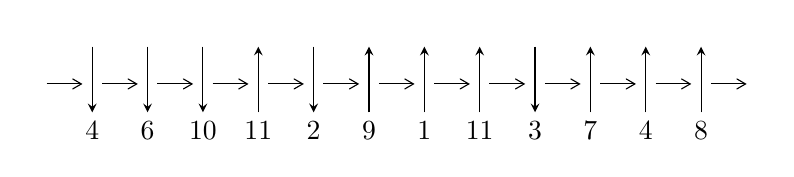
\begin{tikzpicture}[x=20pt, y=17pt]
	% nodes
	\node (C0) at (0, 0) {};
	\node (C1) at (1, 0) {};
	\node (C1U) at (1, +1) {};
	\node (C1D) at (1, -1) {4};

	\node (C2) at (2, 0) {};
	\node (C2U) at (2, +1) {};
	\node (C2D) at (2, -1) {6};

	\node (C3) at (3, 0) {};
	\node (C3U) at (3, +1) {};
	\node (C3D) at (3, -1) {10};

	\node (C4) at (4, 0) {};
	\node (C4U) at (4, +1) {};
	\node (C4D) at (4, -1) {11};

	\node (C5) at (5, 0) {};
	\node (C5U) at (5, +1) {};
	\node (C5D) at (5, -1) {2};

	\node (C6) at (6, 0) {};
	\node (C6U) at (6, +1) {};
	\node (C6D) at (6, -1) {9};

	\node (C7) at (7, 0) {};
	\node (C7U) at (7, +1) {};
	\node (C7D) at (7, -1) {1};

	\node (C8) at (8, 0) {};
	\node (C8U) at (8, +1) {};
	\node (C8D) at (8, -1) {11};

	\node (C9) at (9, 0) {};
	\node (C9U) at (9, +1) {};
	\node (C9D) at (9, -1) {3};

	\node (C10) at (10, 0) {};
	\node (C10U) at (10, +1) {};
	\node (C10D) at (10, -1) {7};

	\node (C11) at (11, 0) {};
	\node (C11U) at (11, +1) {};
	\node (C11D) at (11, -1) {4};

	\node (C12) at (12, 0) {};
	\node (C12U) at (12, +1) {};
	\node (C12D) at (12, -1) {8};
	\node (C13) at (13, 0) {};

	% arrows
	\draw[->,>={angle 60}]
	(C0) edge (C1) (C1) edge (C2) (C2) edge (C3) (C3) edge (C4) (C4) edge (C5) (C5) edge (C6) (C6) edge (C7) (C7) edge (C8) (C8) edge (C9) (C9) edge (C10) (C10) edge (C11) (C11) edge (C12) (C12) edge (C13) ;	\draw[->,>=stealth]
	(C1U) edge (C1D) (C2U) edge (C2D) (C3U) edge (C3D) (C4D) edge (C4U) (C5U) edge (C5D) (C6D) edge (C6U) (C7D) edge (C7U) (C8D) edge (C8U) (C9U) edge (C9D) (C10D) edge (C10U) (C11D) edge (C11U) (C12D) edge (C12U) ;
	\end{tikzpicture} \\
\hhline{~~} \\& 
\textbf{Solving Sequence} \\ \cline{2-2} 
 &
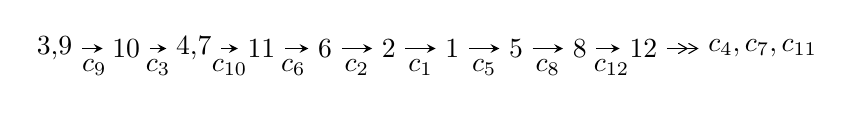
\begin{tikzpicture}[x=23pt, y=7pt]
	% node
	\node (A0) at (-1/8, 0) {3,9};
	\node (A1) at (1, 0) {10};
	\node (A2) at (33/16, 0) {4,7};
	\node (A3) at (25/8, 0) {11};
	\node (A4) at (33/8, 0) {6};
	\node (A5) at (41/8, 0) {2};
	\node (A6) at (49/8, 0) {1};
	\node (A7) at (57/8, 0) {5};
	\node (A8) at (65/8, 0) {8};
	\node (A9) at (73/8, 0) {12};
	\node (C1) at (1/2, -1) {$c_{9}$};
	\node (C2) at (3/2, -1) {$c_{3}$};
	\node (C3) at (21/8, -1) {$c_{10}$};
	\node (C4) at (29/8, -1) {$c_{6}$};
	\node (C5) at (37/8, -1) {$c_{2}$};
	\node (C6) at (45/8, -1) {$c_{1}$};
	\node (C7) at (53/8, -1) {$c_{5}$};
	\node (C8) at (61/8, -1) {$c_{8}$};
	\node (C9) at (69/8, -1) {$c_{12}$};
	\node (A10) at (11, 0) {$c_{4},c_{7},c_{11}$};

	% edge
	\draw[->,>=stealth]	
	(A0) edge (A1) (A1) edge (A2) (A2) edge (A3) (A3) edge (A4) (A4) edge (A5) (A5) edge (A6) (A6) edge (A7) (A7) edge (A8) (A8) edge (A9) ;
	\draw[->>,>={angle 60}]	
	(A9) edge (A10);
\end{tikzpicture} \\ 

\end{tabular} \\

\footnotetext{
The image of knot diagram is generated by the software ``\textbf{Draw programme}" developed by Andrew Bartholomew(\url{http://www.layer8.co.uk/maths/draw/index.htm\#Running-draw}), where we modified some parts for our purpose(\url{https://github.com/CATsTAILs/LinksPainter}).
}\phantom \\ \newline 
\centering \textbf{Ideals for irreducible components\footnotemark of $X_{\text{par}}$} 
 
\begin{align*}
I^u_{1}&=\langle 
8.33978\times10^{205} u^{76}-1.08961\times10^{205} u^{75}+\cdots+1.57363\times10^{205} b+1.04860\times10^{208},\\
\phantom{I^u_{1}}&\phantom{= \langle  }3.39045\times10^{208} u^{76}-4.06453\times10^{207} u^{75}+\cdots+2.18734\times10^{207} a+4.26481\times10^{210},\\
\phantom{I^u_{1}}&\phantom{= \langle  }u^{77}+u^{76}+\cdots+792 u+139\rangle \\
I^u_{2}&=\langle 
91110 u^{16}+162998 u^{15}+\cdots+502439 b+111491,\\
\phantom{I^u_{2}}&\phantom{= \langle  }283556 u^{16}+222982 u^{15}+\cdots+502439 a-280909,\;u^{17}-4 u^{15}+\cdots+4 u^2-1\rangle \\
\\
\end{align*}
\raggedright * 2 irreducible components of $\dim_{\mathbb{C}}=0$, with total 94 representations.\\
\footnotetext{All coefficients of polynomials are rational numbers. But the coefficients are sometimes approximated in decimal forms when there is not enough margin.}
\newpage
\renewcommand{\arraystretch}{1}
\centering \section*{I. $I^u_{1}= \langle 8.34\times10^{205} u^{76}-1.09\times10^{205} u^{75}+\cdots+1.57\times10^{205} b+1.05\times10^{208},\;3.39\times10^{208} u^{76}-4.06\times10^{207} u^{75}+\cdots+2.19\times10^{207} a+4.26\times10^{210},\;u^{77}+u^{76}+\cdots+792 u+139 \rangle$}
\flushleft \textbf{(i) Arc colorings}\\
\begin{tabular}{m{7pt} m{180pt} m{7pt} m{180pt} }
\flushright $a_{3}=$&$\begin{pmatrix}0\\u\end{pmatrix}$ \\
\flushright $a_{9}=$&$\begin{pmatrix}1\\0\end{pmatrix}$ \\
\flushright $a_{10}=$&$\begin{pmatrix}1\\u^2\end{pmatrix}$ \\
\flushright $a_{4}=$&$\begin{pmatrix}- u\\- u^3+u\end{pmatrix}$ \\
\flushright $a_{7}=$&$\begin{pmatrix}-15.5003 u^{76}+1.85821 u^{75}+\cdots-9371.39 u-1949.77\\-5.29972 u^{76}+0.692419 u^{75}+\cdots-3206.91 u-666.357\end{pmatrix}$ \\
\flushright $a_{11}=$&$\begin{pmatrix}61.0416 u^{76}-7.07935 u^{75}+\cdots+36598.3 u+7624.22\\4.27107 u^{76}-0.504359 u^{75}+\cdots+2580.72 u+538.356\end{pmatrix}$ \\
\flushright $a_{6}=$&$\begin{pmatrix}-10.2006 u^{76}+1.16579 u^{75}+\cdots-6164.48 u-1283.41\\-5.29972 u^{76}+0.692419 u^{75}+\cdots-3206.91 u-666.357\end{pmatrix}$ \\
\flushright $a_{2}=$&$\begin{pmatrix}-49.9370 u^{76}+5.72890 u^{75}+\cdots-29859.0 u-6221.64\\-5.17170 u^{76}+0.559340 u^{75}+\cdots-3087.83 u-643.065\end{pmatrix}$ \\
\flushright $a_{1}=$&$\begin{pmatrix}-41.2329 u^{76}+4.69186 u^{75}+\cdots-24646.3 u-5135.91\\-3.01842 u^{76}+0.279790 u^{75}+\cdots-1795.45 u-374.782\end{pmatrix}$ \\
\flushright $a_{5}=$&$\begin{pmatrix}179.435 u^{76}-20.5873 u^{75}+\cdots+107397. u+22372.5\\3.50440 u^{76}-0.359571 u^{75}+\cdots+2115.00 u+440.893\end{pmatrix}$ \\
\flushright $a_{8}=$&$\begin{pmatrix}7.90952 u^{76}-0.847855 u^{75}+\cdots+4713.19 u+984.820\\-1.30653 u^{76}+0.126108 u^{75}+\cdots-789.550 u-164.686\end{pmatrix}$ \\
\flushright $a_{12}=$&$\begin{pmatrix}-47.9834 u^{76}+5.56443 u^{75}+\cdots-28785.0 u-5997.46\\-1.04849 u^{76}+0.133040 u^{75}+\cdots-667.193 u-139.440\end{pmatrix}$\\&\end{tabular}
\flushleft \textbf{(ii) Obstruction class $= -1$}\\~\\
\flushleft \textbf{(iii) Cusp Shapes $= -871.265 u^{76}+100.233 u^{75}+\cdots-521451. u-108615.$}\\~\\
\newpage\renewcommand{\arraystretch}{1}
\flushleft \textbf{(iv) u-Polynomials at the component}\newline \\
\begin{tabular}{m{50pt}|m{274pt}}
Crossings & \hspace{64pt}u-Polynomials at each crossing \\
\hline $$\begin{aligned}c_{1}\end{aligned}$$&$\begin{aligned}
&u^{77}-8 u^{76}+\cdots+32311988 u+2239897
\end{aligned}$\\
\hline $$\begin{aligned}c_{2},c_{5}\end{aligned}$$&$\begin{aligned}
&u^{77}+u^{76}+\cdots-40176 u-5643
\end{aligned}$\\
\hline $$\begin{aligned}c_{3},c_{9}\end{aligned}$$&$\begin{aligned}
&u^{77}+u^{76}+\cdots+792 u+139
\end{aligned}$\\
\hline $$\begin{aligned}c_{4},c_{11}\end{aligned}$$&$\begin{aligned}
&u^{77}-2 u^{76}+\cdots+4508 u-1129
\end{aligned}$\\
\hline $$\begin{aligned}c_{6}\end{aligned}$$&$\begin{aligned}
&u^{77}+3 u^{76}+\cdots-2292 u-319
\end{aligned}$\\
\hline $$\begin{aligned}c_{7},c_{12}\end{aligned}$$&$\begin{aligned}
&u^{77}- u^{76}+\cdots-37 u-11
\end{aligned}$\\
\hline $$\begin{aligned}c_{8}\end{aligned}$$&$\begin{aligned}
&u^{77}+6 u^{76}+\cdots+195 u-19
\end{aligned}$\\
\hline $$\begin{aligned}c_{10}\end{aligned}$$&$\begin{aligned}
&u^{77}- u^{76}+\cdots-15 u-1
\end{aligned}$\\
\hline
\end{tabular}\\~\\
\newpage\renewcommand{\arraystretch}{1}
\flushleft \textbf{(v) Riley Polynomials at the component}\newline \\
\begin{tabular}{m{50pt}|m{274pt}}
Crossings & \hspace{64pt}Riley Polynomials at each crossing \\
\hline $$\begin{aligned}c_{1}\end{aligned}$$&$\begin{aligned}
&y^{77}+44 y^{76}+\cdots+727248075963258 y-5017138570609
\end{aligned}$\\
\hline $$\begin{aligned}c_{2},c_{5}\end{aligned}$$&$\begin{aligned}
&y^{77}-63 y^{76}+\cdots+793460772 y-31843449
\end{aligned}$\\
\hline $$\begin{aligned}c_{3},c_{9}\end{aligned}$$&$\begin{aligned}
&y^{77}-51 y^{76}+\cdots+189414 y-19321
\end{aligned}$\\
\hline $$\begin{aligned}c_{4},c_{11}\end{aligned}$$&$\begin{aligned}
&y^{77}-66 y^{76}+\cdots+58868382 y-1274641
\end{aligned}$\\
\hline $$\begin{aligned}c_{6}\end{aligned}$$&$\begin{aligned}
&y^{77}+23 y^{76}+\cdots-2243236 y-101761
\end{aligned}$\\
\hline $$\begin{aligned}c_{7},c_{12}\end{aligned}$$&$\begin{aligned}
&y^{77}+25 y^{76}+\cdots-2041 y-121
\end{aligned}$\\
\hline $$\begin{aligned}c_{8}\end{aligned}$$&$\begin{aligned}
&y^{77}-108 y^{76}+\cdots+382001 y-361
\end{aligned}$\\
\hline $$\begin{aligned}c_{10}\end{aligned}$$&$\begin{aligned}
&y^{77}-19 y^{76}+\cdots-25 y-1
\end{aligned}$\\
\hline
\end{tabular}\\~\\
\newpage\flushleft \textbf{(vi) Complex Volumes and Cusp Shapes}
$$\begin{array}{c|c|c}  
\text{Solutions to }I^u_{1}& \I (\text{vol} + \sqrt{-1}CS) & \text{Cusp shape}\\
 \hline 
\begin{aligned}
u &= -0.758997 + 0.616342 I \\
a &= \phantom{-}1.46817 - 0.34902 I \\
b &= \phantom{-}0.79967 - 1.26583 I\end{aligned}
 & \phantom{-}1.32991 - 1.97035 I & \phantom{-0.000000 } 0 \\ \hline\begin{aligned}
u &= -0.758997 - 0.616342 I \\
a &= \phantom{-}1.46817 + 0.34902 I \\
b &= \phantom{-}0.79967 + 1.26583 I\end{aligned}
 & \phantom{-}1.32991 + 1.97035 I & \phantom{-0.000000 } 0 \\ \hline\begin{aligned}
u &= \phantom{-}0.911703\phantom{ +0.000000I} \\
a &= \phantom{-}1.42882\phantom{ +0.000000I} \\
b &= \phantom{-}2.17200\phantom{ +0.000000I}\end{aligned}
 & \phantom{-}3.05365\phantom{ +0.000000I} & \phantom{-0.000000 } 0 \\ \hline\begin{aligned}
u &= -0.010819 + 1.090530 I \\
a &= \phantom{-}0.191191 - 0.124778 I \\
b &= \phantom{-}0.734597 + 0.849848 I\end{aligned}
 & \phantom{-}4.01664 + 4.54282 I & \phantom{-0.000000 } 0 \\ \hline\begin{aligned}
u &= -0.010819 - 1.090530 I \\
a &= \phantom{-}0.191191 + 0.124778 I \\
b &= \phantom{-}0.734597 - 0.849848 I\end{aligned}
 & \phantom{-}4.01664 - 4.54282 I & \phantom{-0.000000 } 0 \\ \hline\begin{aligned}
u &= -1.065640 + 0.254276 I \\
a &= \phantom{-}0.480002 - 1.159030 I \\
b &= -0.292883 - 0.664587 I\end{aligned}
 & -1.91191 + 1.13599 I & \phantom{-0.000000 } 0 \\ \hline\begin{aligned}
u &= -1.065640 - 0.254276 I \\
a &= \phantom{-}0.480002 + 1.159030 I \\
b &= -0.292883 + 0.664587 I\end{aligned}
 & -1.91191 - 1.13599 I & \phantom{-0.000000 } 0 \\ \hline\begin{aligned}
u &= -1.11487\phantom{ +0.000000I} \\
a &= -2.43271\phantom{ +0.000000I} \\
b &= \phantom{-}0.374887\phantom{ +0.000000I}\end{aligned}
 & -3.74100\phantom{ +0.000000I} & \phantom{-0.000000 } 0 \\ \hline\begin{aligned}
u &= -1.116270 + 0.007414 I \\
a &= -0.620793 - 0.148394 I \\
b &= \phantom{-}1.005310 - 0.198862 I\end{aligned}
 & -3.83080 + 0.35334 I & \phantom{-0.000000 } 0 \\ \hline\begin{aligned}
u &= -1.116270 - 0.007414 I \\
a &= -0.620793 + 0.148394 I \\
b &= \phantom{-}1.005310 + 0.198862 I\end{aligned}
 & -3.83080 - 0.35334 I & \phantom{-0.000000 } 0\\
 \hline 
 \end{array}$$\newpage$$\begin{array}{c|c|c}  
\text{Solutions to }I^u_{1}& \I (\text{vol} + \sqrt{-1}CS) & \text{Cusp shape}\\
 \hline 
\begin{aligned}
u &= -0.695591 + 0.874541 I \\
a &= -0.104081 - 0.102779 I \\
b &= -0.528202 - 0.116523 I\end{aligned}
 & -0.95380 + 2.56825 I & \phantom{-0.000000 } 0 \\ \hline\begin{aligned}
u &= -0.695591 - 0.874541 I \\
a &= -0.104081 + 0.102779 I \\
b &= -0.528202 + 0.116523 I\end{aligned}
 & -0.95380 - 2.56825 I & \phantom{-0.000000 } 0 \\ \hline\begin{aligned}
u &= -1.119770 + 0.088439 I \\
a &= -1.30975 + 1.24365 I \\
b &= -2.25028 + 1.34716 I\end{aligned}
 & -0.31477 + 6.50480 I & \phantom{-0.000000 } 0 \\ \hline\begin{aligned}
u &= -1.119770 - 0.088439 I \\
a &= -1.30975 - 1.24365 I \\
b &= -2.25028 - 1.34716 I\end{aligned}
 & -0.31477 - 6.50480 I & \phantom{-0.000000 } 0 \\ \hline\begin{aligned}
u &= \phantom{-}1.103770 + 0.223227 I \\
a &= \phantom{-}0.322545 + 0.190472 I \\
b &= -0.960347 + 0.441859 I\end{aligned}
 & -6.03076 - 3.62911 I & \phantom{-0.000000 } 0 \\ \hline\begin{aligned}
u &= \phantom{-}1.103770 - 0.223227 I \\
a &= \phantom{-}0.322545 - 0.190472 I \\
b &= -0.960347 - 0.441859 I\end{aligned}
 & -6.03076 + 3.62911 I & \phantom{-0.000000 } 0 \\ \hline\begin{aligned}
u &= \phantom{-}1.035260 + 0.465565 I \\
a &= -1.16999 - 1.22271 I \\
b &= -0.62849 - 1.67436 I\end{aligned}
 & \phantom{-}0.58777 - 4.71952 I & \phantom{-0.000000 } 0 \\ \hline\begin{aligned}
u &= \phantom{-}1.035260 - 0.465565 I \\
a &= -1.16999 + 1.22271 I \\
b &= -0.62849 + 1.67436 I\end{aligned}
 & \phantom{-}0.58777 + 4.71952 I & \phantom{-0.000000 } 0 \\ \hline\begin{aligned}
u &= \phantom{-}0.217467 + 0.833274 I \\
a &= \phantom{-}0.204278 - 0.401189 I \\
b &= -1.035260 - 0.397841 I\end{aligned}
 & \phantom{-}5.89269 + 5.41568 I & \phantom{-0.000000 } 0 \\ \hline\begin{aligned}
u &= \phantom{-}0.217467 - 0.833274 I \\
a &= \phantom{-}0.204278 + 0.401189 I \\
b &= -1.035260 + 0.397841 I\end{aligned}
 & \phantom{-}5.89269 - 5.41568 I & \phantom{-0.000000 } 0\\
 \hline 
 \end{array}$$\newpage$$\begin{array}{c|c|c}  
\text{Solutions to }I^u_{1}& \I (\text{vol} + \sqrt{-1}CS) & \text{Cusp shape}\\
 \hline 
\begin{aligned}
u &= \phantom{-}1.091030 + 0.347422 I \\
a &= -0.11223 - 1.63823 I \\
b &= \phantom{-}0.494694 - 1.137330 I\end{aligned}
 & -1.10617 - 4.08847 I & \phantom{-0.000000 } 0 \\ \hline\begin{aligned}
u &= \phantom{-}1.091030 - 0.347422 I \\
a &= -0.11223 + 1.63823 I \\
b &= \phantom{-}0.494694 + 1.137330 I\end{aligned}
 & -1.10617 + 4.08847 I & \phantom{-0.000000 } 0 \\ \hline\begin{aligned}
u &= -1.116810 + 0.335012 I \\
a &= \phantom{-}0.40003 + 1.95228 I \\
b &= \phantom{-}0.565199 + 0.678583 I\end{aligned}
 & \phantom{-}3.30736 + 2.92566 I & \phantom{-0.000000 } 0 \\ \hline\begin{aligned}
u &= -1.116810 - 0.335012 I \\
a &= \phantom{-}0.40003 - 1.95228 I \\
b &= \phantom{-}0.565199 - 0.678583 I\end{aligned}
 & \phantom{-}3.30736 - 2.92566 I & \phantom{-0.000000 } 0 \\ \hline\begin{aligned}
u &= \phantom{-}1.181340 + 0.003850 I \\
a &= -0.92722 + 1.76444 I \\
b &= -0.134594 + 1.072470 I\end{aligned}
 & -7.66719 - 1.85639 I & \phantom{-0.000000 } 0 \\ \hline\begin{aligned}
u &= \phantom{-}1.181340 - 0.003850 I \\
a &= -0.92722 - 1.76444 I \\
b &= -0.134594 - 1.072470 I\end{aligned}
 & -7.66719 + 1.85639 I & \phantom{-0.000000 } 0 \\ \hline\begin{aligned}
u &= -1.183980 + 0.202308 I \\
a &= \phantom{-}0.82439 - 1.52658 I \\
b &= -0.452462 - 0.812176 I\end{aligned}
 & -1.38098 + 1.72001 I & \phantom{-0.000000 } 0 \\ \hline\begin{aligned}
u &= -1.183980 - 0.202308 I \\
a &= \phantom{-}0.82439 + 1.52658 I \\
b &= -0.452462 + 0.812176 I\end{aligned}
 & -1.38098 - 1.72001 I & \phantom{-0.000000 } 0 \\ \hline\begin{aligned}
u &= \phantom{-}0.787886 + 0.099348 I \\
a &= \phantom{-}1.52773 - 2.14738 I \\
b &= \phantom{-}1.01856 - 1.19509 I\end{aligned}
 & \phantom{-}3.17288 - 1.22575 I & \phantom{-0.000000 } 0 \\ \hline\begin{aligned}
u &= \phantom{-}0.787886 - 0.099348 I \\
a &= \phantom{-}1.52773 + 2.14738 I \\
b &= \phantom{-}1.01856 + 1.19509 I\end{aligned}
 & \phantom{-}3.17288 + 1.22575 I & \phantom{-0.000000 } 0\\
 \hline 
 \end{array}$$\newpage$$\begin{array}{c|c|c}  
\text{Solutions to }I^u_{1}& \I (\text{vol} + \sqrt{-1}CS) & \text{Cusp shape}\\
 \hline 
\begin{aligned}
u &= \phantom{-}0.000804 + 1.208190 I \\
a &= \phantom{-}0.216880 + 0.347898 I \\
b &= \phantom{-}0.225684 - 0.704296 I\end{aligned}
 & -3.05027 - 0.94756 I & \phantom{-0.000000 } 0 \\ \hline\begin{aligned}
u &= \phantom{-}0.000804 - 1.208190 I \\
a &= \phantom{-}0.216880 - 0.347898 I \\
b &= \phantom{-}0.225684 + 0.704296 I\end{aligned}
 & -3.05027 + 0.94756 I & \phantom{-0.000000 } 0 \\ \hline\begin{aligned}
u &= \phantom{-}0.133250 + 1.220520 I \\
a &= -0.131494 - 0.101763 I \\
b &= -0.694787 + 0.844760 I\end{aligned}
 & \phantom{-}2.85374 - 11.06360 I & \phantom{-0.000000 } 0 \\ \hline\begin{aligned}
u &= \phantom{-}0.133250 - 1.220520 I \\
a &= -0.131494 + 0.101763 I \\
b &= -0.694787 - 0.844760 I\end{aligned}
 & \phantom{-}2.85374 + 11.06360 I & \phantom{-0.000000 } 0 \\ \hline\begin{aligned}
u &= -0.722758 + 0.238117 I \\
a &= -1.75262 + 2.18724 I \\
b &= -0.21833 + 1.90963 I\end{aligned}
 & \phantom{-}1.55815 + 6.08582 I & \phantom{-0.000000 } 0 \\ \hline\begin{aligned}
u &= -0.722758 - 0.238117 I \\
a &= -1.75262 - 2.18724 I \\
b &= -0.21833 - 1.90963 I\end{aligned}
 & \phantom{-}1.55815 - 6.08582 I & \phantom{-0.000000 } 0 \\ \hline\begin{aligned}
u &= \phantom{-}0.755834\phantom{ +0.000000I} \\
a &= \phantom{-}1.17517\phantom{ +0.000000I} \\
b &= \phantom{-}1.75003\phantom{ +0.000000I}\end{aligned}
 & \phantom{-}3.09798\phantom{ +0.000000I} & -4.83340\phantom{ +0.000000I} \\ \hline\begin{aligned}
u &= \phantom{-}1.172280 + 0.417636 I \\
a &= -0.17453 + 1.80364 I \\
b &= -0.661781 + 0.694578 I\end{aligned}
 & \phantom{-}2.92989 - 9.94785 I & \phantom{-0.000000 } 0 \\ \hline\begin{aligned}
u &= \phantom{-}1.172280 - 0.417636 I \\
a &= -0.17453 - 1.80364 I \\
b &= -0.661781 - 0.694578 I\end{aligned}
 & \phantom{-}2.92989 + 9.94785 I & \phantom{-0.000000 } 0 \\ \hline\begin{aligned}
u &= \phantom{-}1.272770 + 0.184016 I \\
a &= -0.65660 - 1.47391 I \\
b &= \phantom{-}0.651251 - 0.990914 I\end{aligned}
 & -3.05844 - 8.07962 I & \phantom{-0.000000 } 0\\
 \hline 
 \end{array}$$\newpage$$\begin{array}{c|c|c}  
\text{Solutions to }I^u_{1}& \I (\text{vol} + \sqrt{-1}CS) & \text{Cusp shape}\\
 \hline 
\begin{aligned}
u &= \phantom{-}1.272770 - 0.184016 I \\
a &= -0.65660 + 1.47391 I \\
b &= \phantom{-}0.651251 + 0.990914 I\end{aligned}
 & -3.05844 + 8.07962 I & \phantom{-0.000000 } 0 \\ \hline\begin{aligned}
u &= -0.290588 + 0.637778 I \\
a &= -0.311030 - 0.501017 I \\
b &= \phantom{-}1.131460 - 0.351988 I\end{aligned}
 & \phantom{-}5.82765 + 0.77594 I & \phantom{-}5.84300 - 2.67611 I \\ \hline\begin{aligned}
u &= -0.290588 - 0.637778 I \\
a &= -0.311030 + 0.501017 I \\
b &= \phantom{-}1.131460 + 0.351988 I\end{aligned}
 & \phantom{-}5.82765 - 0.77594 I & \phantom{-}5.84300 + 2.67611 I \\ \hline\begin{aligned}
u &= \phantom{-}1.300670 + 0.104807 I \\
a &= \phantom{-}0.145206 - 1.109260 I \\
b &= -0.578994 - 0.801863 I\end{aligned}
 & -6.47566 - 2.58505 I & \phantom{-0.000000 } 0 \\ \hline\begin{aligned}
u &= \phantom{-}1.300670 - 0.104807 I \\
a &= \phantom{-}0.145206 + 1.109260 I \\
b &= -0.578994 + 0.801863 I\end{aligned}
 & -6.47566 + 2.58505 I & \phantom{-0.000000 } 0 \\ \hline\begin{aligned}
u &= -0.638923 + 0.237400 I \\
a &= \phantom{-}1.92039 - 0.14693 I \\
b &= -0.213109 - 0.365332 I\end{aligned}
 & -2.17556 + 0.65395 I & -9.20343 - 5.27465 I \\ \hline\begin{aligned}
u &= -0.638923 - 0.237400 I \\
a &= \phantom{-}1.92039 + 0.14693 I \\
b &= -0.213109 + 0.365332 I\end{aligned}
 & -2.17556 - 0.65395 I & -9.20343 + 5.27465 I \\ \hline\begin{aligned}
u &= -1.291130 + 0.352756 I \\
a &= -0.02607 - 1.87165 I \\
b &= -0.88563 - 1.75280 I\end{aligned}
 & -8.67471 + 6.59602 I & \phantom{-0.000000 } 0 \\ \hline\begin{aligned}
u &= -1.291130 - 0.352756 I \\
a &= -0.02607 + 1.87165 I \\
b &= -0.88563 + 1.75280 I\end{aligned}
 & -8.67471 - 6.59602 I & \phantom{-0.000000 } 0 \\ \hline\begin{aligned}
u &= \phantom{-}0.330805 + 0.513963 I \\
a &= \phantom{-}0.447914 - 0.085197 I \\
b &= \phantom{-}0.633023 + 0.390219 I\end{aligned}
 & \phantom{-}1.170010 + 0.511271 I & \phantom{-}7.93499 - 2.10183 I\\
 \hline 
 \end{array}$$\newpage$$\begin{array}{c|c|c}  
\text{Solutions to }I^u_{1}& \I (\text{vol} + \sqrt{-1}CS) & \text{Cusp shape}\\
 \hline 
\begin{aligned}
u &= \phantom{-}0.330805 - 0.513963 I \\
a &= \phantom{-}0.447914 + 0.085197 I \\
b &= \phantom{-}0.633023 - 0.390219 I\end{aligned}
 & \phantom{-}1.170010 - 0.511271 I & \phantom{-}7.93499 + 2.10183 I \\ \hline\begin{aligned}
u &= \phantom{-}0.246079 + 0.526147 I \\
a &= \phantom{-}1.57072 + 0.38139 I \\
b &= -0.025841 + 1.081900 I\end{aligned}
 & \phantom{-}2.60807 + 0.74898 I & \phantom{-}3.51716 - 0.31657 I \\ \hline\begin{aligned}
u &= \phantom{-}0.246079 - 0.526147 I \\
a &= \phantom{-}1.57072 - 0.38139 I \\
b &= -0.025841 - 1.081900 I\end{aligned}
 & \phantom{-}2.60807 - 0.74898 I & \phantom{-}3.51716 + 0.31657 I \\ \hline\begin{aligned}
u &= \phantom{-}1.35457 + 0.52174 I \\
a &= -0.01207 - 1.55989 I \\
b &= \phantom{-}1.02876 - 1.43648 I\end{aligned}
 & -0.26091 - 10.21520 I & \phantom{-0.000000 } 0 \\ \hline\begin{aligned}
u &= \phantom{-}1.35457 - 0.52174 I \\
a &= -0.01207 + 1.55989 I \\
b &= \phantom{-}1.02876 + 1.43648 I\end{aligned}
 & -0.26091 + 10.21520 I & \phantom{-0.000000 } 0 \\ \hline\begin{aligned}
u &= \phantom{-}0.080850 + 0.537512 I \\
a &= -0.331378 - 0.654699 I \\
b &= -0.707167 + 0.980733 I\end{aligned}
 & -4.48701 - 3.03669 I & \phantom{-}5.16104 + 7.39684 I \\ \hline\begin{aligned}
u &= \phantom{-}0.080850 - 0.537512 I \\
a &= -0.331378 + 0.654699 I \\
b &= -0.707167 - 0.980733 I\end{aligned}
 & -4.48701 + 3.03669 I & \phantom{-}5.16104 - 7.39684 I \\ \hline\begin{aligned}
u &= \phantom{-}1.40085 + 0.40250 I \\
a &= -0.016309 + 1.193430 I \\
b &= -1.04169 + 1.29261 I\end{aligned}
 & -8.68571 - 4.73560 I & \phantom{-0.000000 } 0 \\ \hline\begin{aligned}
u &= \phantom{-}1.40085 - 0.40250 I \\
a &= -0.016309 - 1.193430 I \\
b &= -1.04169 - 1.29261 I\end{aligned}
 & -8.68571 + 4.73560 I & \phantom{-0.000000 } 0 \\ \hline\begin{aligned}
u &= -1.39036 + 0.57949 I \\
a &= -0.159041 + 1.141650 I \\
b &= \phantom{-}0.77534 + 1.38516 I\end{aligned}
 & -7.31609 + 7.24715 I & \phantom{-0.000000 } 0\\
 \hline 
 \end{array}$$\newpage$$\begin{array}{c|c|c}  
\text{Solutions to }I^u_{1}& \I (\text{vol} + \sqrt{-1}CS) & \text{Cusp shape}\\
 \hline 
\begin{aligned}
u &= -1.39036 - 0.57949 I \\
a &= -0.159041 - 1.141650 I \\
b &= \phantom{-}0.77534 - 1.38516 I\end{aligned}
 & -7.31609 - 7.24715 I & \phantom{-0.000000 } 0 \\ \hline\begin{aligned}
u &= -0.394801 + 0.288987 I \\
a &= -2.66235 + 1.07859 I \\
b &= -0.152342 + 1.354640 I\end{aligned}
 & \phantom{-}1.61463 + 6.08143 I & \phantom{-}1.65363 - 3.54096 I \\ \hline\begin{aligned}
u &= -0.394801 - 0.288987 I \\
a &= -2.66235 - 1.07859 I \\
b &= -0.152342 - 1.354640 I\end{aligned}
 & \phantom{-}1.61463 - 6.08143 I & \phantom{-}1.65363 + 3.54096 I \\ \hline\begin{aligned}
u &= -1.42831 + 0.53758 I \\
a &= -0.03870 - 1.46221 I \\
b &= -1.09850 - 1.41506 I\end{aligned}
 & -2.0258 + 17.1703 I & \phantom{-0.000000 } 0 \\ \hline\begin{aligned}
u &= -1.42831 - 0.53758 I \\
a &= -0.03870 + 1.46221 I \\
b &= -1.09850 + 1.41506 I\end{aligned}
 & -2.0258 - 17.1703 I & \phantom{-0.000000 } 0 \\ \hline\begin{aligned}
u &= \phantom{-}1.46502 + 0.49693 I \\
a &= \phantom{-}0.037413 + 1.171880 I \\
b &= -0.853847 + 1.061410 I\end{aligned}
 & -7.05974 - 8.63532 I & \phantom{-0.000000 } 0 \\ \hline\begin{aligned}
u &= \phantom{-}1.46502 - 0.49693 I \\
a &= \phantom{-}0.037413 - 1.171880 I \\
b &= -0.853847 - 1.061410 I\end{aligned}
 & -7.05974 + 8.63532 I & \phantom{-0.000000 } 0 \\ \hline\begin{aligned}
u &= -1.50322 + 0.49069 I \\
a &= \phantom{-}0.006370 + 1.080770 I \\
b &= \phantom{-}0.677127 + 1.140250 I\end{aligned}
 & -7.01071 + 4.87145 I & \phantom{-0.000000 } 0 \\ \hline\begin{aligned}
u &= -1.50322 - 0.49069 I \\
a &= \phantom{-}0.006370 - 1.080770 I \\
b &= \phantom{-}0.677127 - 1.140250 I\end{aligned}
 & -7.01071 - 4.87145 I & \phantom{-0.000000 } 0 \\ \hline\begin{aligned}
u &= -0.210525 + 0.311466 I \\
a &= \phantom{-}2.18028 + 1.43772 I \\
b &= -0.206538 + 0.269662 I\end{aligned}
 & -1.90333 + 0.92139 I & -5.44582 + 1.92407 I\\
 \hline 
 \end{array}$$\newpage$$\begin{array}{c|c|c}  
\text{Solutions to }I^u_{1}& \I (\text{vol} + \sqrt{-1}CS) & \text{Cusp shape}\\
 \hline 
\begin{aligned}
u &= -0.210525 - 0.311466 I \\
a &= \phantom{-}2.18028 - 1.43772 I \\
b &= -0.206538 - 0.269662 I\end{aligned}
 & -1.90333 - 0.92139 I & -5.44582 - 1.92407 I \\ \hline\begin{aligned}
u &= -1.70360 + 0.29340 I \\
a &= \phantom{-}0.021683 - 0.365141 I \\
b &= -0.406453 - 0.522497 I\end{aligned}
 & -0.79210 + 1.62218 I & \phantom{-0.000000 } 0 \\ \hline\begin{aligned}
u &= -1.70360 - 0.29340 I \\
a &= \phantom{-}0.021683 + 0.365141 I \\
b &= -0.406453 + 0.522497 I\end{aligned}
 & -0.79210 - 1.62218 I & \phantom{-0.000000 } 0 \\ \hline\begin{aligned}
u &= \phantom{-}1.94427 + 0.25926 I \\
a &= \phantom{-}0.191630 - 0.307980 I \\
b &= \phantom{-}0.708436 - 0.462080 I\end{aligned}
 & -1.70623 + 3.05877 I & \phantom{-0.000000 } 0 \\ \hline\begin{aligned}
u &= \phantom{-}1.94427 - 0.25926 I \\
a &= \phantom{-}0.191630 + 0.307980 I \\
b &= \phantom{-}0.708436 + 0.462080 I\end{aligned}
 & -1.70623 - 3.05877 I & \phantom{-0.000000 } 0 \\ \hline\begin{aligned}
u &= -0.25319 + 2.28522 I \\
a &= \phantom{-}0.0183860 + 0.0150818 I \\
b &= -0.070031 - 0.348268 I\end{aligned}
 & -1.18900 + 2.18789 I & \phantom{-0.000000 } 0 \\ \hline\begin{aligned}
u &= -0.25319 - 2.28522 I \\
a &= \phantom{-}0.0183860 - 0.0150818 I \\
b &= -0.070031 + 0.348268 I\end{aligned}
 & -1.18900 - 2.18789 I & \phantom{-0.000000 } 0\\
 \hline 
 \end{array}$$\newpage\newpage\renewcommand{\arraystretch}{1}
\centering \section*{II. $I^u_{2}= \langle 9.11\times10^{4} u^{16}+1.63\times10^{5} u^{15}+\cdots+5.02\times10^{5} b+1.11\times10^{5},\;2.84\times10^{5} u^{16}+2.23\times10^{5} u^{15}+\cdots+5.02\times10^{5} a-2.81\times10^{5},\;u^{17}-4 u^{15}+\cdots+4 u^2-1 \rangle$}
\flushleft \textbf{(i) Arc colorings}\\
\begin{tabular}{m{7pt} m{180pt} m{7pt} m{180pt} }
\flushright $a_{3}=$&$\begin{pmatrix}0\\u\end{pmatrix}$ \\
\flushright $a_{9}=$&$\begin{pmatrix}1\\0\end{pmatrix}$ \\
\flushright $a_{10}=$&$\begin{pmatrix}1\\u^2\end{pmatrix}$ \\
\flushright $a_{4}=$&$\begin{pmatrix}- u\\- u^3+u\end{pmatrix}$ \\
\flushright $a_{7}=$&$\begin{pmatrix}-0.564359 u^{16}-0.443799 u^{15}+\cdots+0.499613 u+0.559091\\-0.181335 u^{16}-0.324414 u^{15}+\cdots+1.71782 u-0.221900\end{pmatrix}$ \\
\flushright $a_{11}=$&$\begin{pmatrix}-0.523656 u^{16}+1.25267 u^{15}+\cdots-0.706948 u+0.869208\\-0.166132 u^{16}+0.102498 u^{15}+\cdots-2.58379 u-1.39833\end{pmatrix}$ \\
\flushright $a_{6}=$&$\begin{pmatrix}-0.383024 u^{16}-0.119386 u^{15}+\cdots-1.21821 u+0.780990\\-0.181335 u^{16}-0.324414 u^{15}+\cdots+1.71782 u-0.221900\end{pmatrix}$ \\
\flushright $a_{2}=$&$\begin{pmatrix}0.166693 u^{16}-0.255010 u^{15}+\cdots+0.0329612 u-2.12171\\-1.18134 u^{16}-0.324414 u^{15}+\cdots-1.28218 u-0.221900\end{pmatrix}$ \\
\flushright $a_{1}=$&$\begin{pmatrix}-0.979729 u^{16}-0.559953 u^{15}+\cdots-1.43071 u-3.07725\\-0.565850 u^{16}-0.255541 u^{15}+\cdots-0.964933 u+0.428689\end{pmatrix}$ \\
\flushright $a_{5}=$&$\begin{pmatrix}-2.22373 u^{16}-2.33836 u^{15}+\cdots-2.59451 u-3.02392\\0.499460 u^{16}+0.149873 u^{15}+\cdots+3.16482 u+0.900376\end{pmatrix}$ \\
\flushright $a_{8}=$&$\begin{pmatrix}0.552909 u^{16}-0.722456 u^{15}+\cdots-2.87988 u+1.54459\\0.787403 u^{16}+0.296938 u^{15}+\cdots+5.41888 u+0.897773\end{pmatrix}$ \\
\flushright $a_{12}=$&$\begin{pmatrix}-0.404270 u^{16}+1.13515 u^{15}+\cdots-1.48794 u+0.252232\\-0.0162587 u^{16}+0.0532403 u^{15}+\cdots-1.68341 u-0.898869\end{pmatrix}$\\&\end{tabular}
\flushleft \textbf{(ii) Obstruction class $= 1$}\\~\\
\flushleft \textbf{(iii) Cusp Shapes $= \frac{7310202}{502439} u^{16}+\frac{3456735}{502439} u^{15}+\cdots+\frac{15933523}{502439} u+\frac{5895545}{502439}$}\\~\\
\newpage\renewcommand{\arraystretch}{1}
\flushleft \textbf{(iv) u-Polynomials at the component}\newline \\
\begin{tabular}{m{50pt}|m{274pt}}
Crossings & \hspace{64pt}u-Polynomials at each crossing \\
\hline $$\begin{aligned}c_{1}\end{aligned}$$&$\begin{aligned}
&u^{17}+3 u^{16}+\cdots-94 u+31
\end{aligned}$\\
\hline $$\begin{aligned}c_{2}\end{aligned}$$&$\begin{aligned}
&u^{17}+6 u^{16}+\cdots+12 u+5
\end{aligned}$\\
\hline $$\begin{aligned}c_{3}\end{aligned}$$&$\begin{aligned}
&u^{17}-4 u^{15}+\cdots-4 u^2+1
\end{aligned}$\\
\hline $$\begin{aligned}c_{4}\end{aligned}$$&$\begin{aligned}
&u^{17}+u^{16}+\cdots+6 u-1
\end{aligned}$\\
\hline $$\begin{aligned}c_{5}\end{aligned}$$&$\begin{aligned}
&u^{17}-6 u^{16}+\cdots+12 u-5
\end{aligned}$\\
\hline $$\begin{aligned}c_{6}\end{aligned}$$&$\begin{aligned}
&u^{17}+3 u^{15}+\cdots-2 u-1
\end{aligned}$\\
\hline $$\begin{aligned}c_{7}\end{aligned}$$&$\begin{aligned}
&u^{17}-2 u^{16}+\cdots+u-1
\end{aligned}$\\
\hline $$\begin{aligned}c_{8}\end{aligned}$$&$\begin{aligned}
&u^{17}+7 u^{16}+\cdots+221 u+23
\end{aligned}$\\
\hline $$\begin{aligned}c_{9}\end{aligned}$$&$\begin{aligned}
&u^{17}-4 u^{15}+\cdots+4 u^2-1
\end{aligned}$\\
\hline $$\begin{aligned}c_{10}\end{aligned}$$&$\begin{aligned}
&u^{17}-8 u^{15}+\cdots- u+1
\end{aligned}$\\
\hline $$\begin{aligned}c_{11}\end{aligned}$$&$\begin{aligned}
&u^{17}- u^{16}+\cdots+6 u+1
\end{aligned}$\\
\hline $$\begin{aligned}c_{12}\end{aligned}$$&$\begin{aligned}
&u^{17}+2 u^{16}+\cdots+u+1
\end{aligned}$\\
\hline
\end{tabular}\\~\\
\newpage\renewcommand{\arraystretch}{1}
\flushleft \textbf{(v) Riley Polynomials at the component}\newline \\
\begin{tabular}{m{50pt}|m{274pt}}
Crossings & \hspace{64pt}Riley Polynomials at each crossing \\
\hline $$\begin{aligned}c_{1}\end{aligned}$$&$\begin{aligned}
&y^{17}-5 y^{16}+\cdots-11376 y-961
\end{aligned}$\\
\hline $$\begin{aligned}c_{2},c_{5}\end{aligned}$$&$\begin{aligned}
&y^{17}-28 y^{16}+\cdots-6 y-25
\end{aligned}$\\
\hline $$\begin{aligned}c_{3},c_{9}\end{aligned}$$&$\begin{aligned}
&y^{17}-8 y^{16}+\cdots+8 y-1
\end{aligned}$\\
\hline $$\begin{aligned}c_{4},c_{11}\end{aligned}$$&$\begin{aligned}
&y^{17}-7 y^{16}+\cdots+24 y-1
\end{aligned}$\\
\hline $$\begin{aligned}c_{6}\end{aligned}$$&$\begin{aligned}
&y^{17}+6 y^{16}+\cdots-14 y-1
\end{aligned}$\\
\hline $$\begin{aligned}c_{7},c_{12}\end{aligned}$$&$\begin{aligned}
&y^{17}+12 y^{16}+\cdots-3 y-1
\end{aligned}$\\
\hline $$\begin{aligned}c_{8}\end{aligned}$$&$\begin{aligned}
&y^{17}-5 y^{16}+\cdots+20459 y-529
\end{aligned}$\\
\hline $$\begin{aligned}c_{10}\end{aligned}$$&$\begin{aligned}
&y^{17}-16 y^{16}+\cdots-43 y-1
\end{aligned}$\\
\hline
\end{tabular}\\~\\
\newpage\flushleft \textbf{(vi) Complex Volumes and Cusp Shapes}
$$\begin{array}{c|c|c}  
\text{Solutions to }I^u_{2}& \I (\text{vol} + \sqrt{-1}CS) & \text{Cusp shape}\\
 \hline 
\begin{aligned}
u &= \phantom{-}1.10570\phantom{ +0.000000I} \\
a &= \phantom{-}2.70999\phantom{ +0.000000I} \\
b &= -0.375089\phantom{ +0.000000I}\end{aligned}
 & -3.71205\phantom{ +0.000000I} & \phantom{-}178.710\phantom{ +0.000000I} \\ \hline\begin{aligned}
u &= -0.852456 + 0.254240 I \\
a &= -2.20438 + 2.03152 I \\
b &= -1.12246 + 1.74335 I\end{aligned}
 & \phantom{-}1.30681 + 6.74725 I & \phantom{-}1.14602 - 11.82219 I \\ \hline\begin{aligned}
u &= -0.852456 - 0.254240 I \\
a &= -2.20438 - 2.03152 I \\
b &= -1.12246 - 1.74335 I\end{aligned}
 & \phantom{-}1.30681 - 6.74725 I & \phantom{-}1.14602 + 11.82219 I \\ \hline\begin{aligned}
u &= -1.231690 + 0.050913 I \\
a &= -0.72795 - 1.70057 I \\
b &= \phantom{-}0.078174 - 1.030070 I\end{aligned}
 & -8.23055 + 2.35568 I & -10.79846 - 4.11130 I \\ \hline\begin{aligned}
u &= -1.231690 - 0.050913 I \\
a &= -0.72795 + 1.70057 I \\
b &= \phantom{-}0.078174 + 1.030070 I\end{aligned}
 & -8.23055 - 2.35568 I & -10.79846 + 4.11130 I \\ \hline\begin{aligned}
u &= \phantom{-}0.566286 + 0.419821 I \\
a &= -1.35242 + 0.75569 I \\
b &= \phantom{-}0.441137 - 0.361394 I\end{aligned}
 & -1.78451 + 0.00683 I & \phantom{-}1.85797 - 0.92831 I \\ \hline\begin{aligned}
u &= \phantom{-}0.566286 - 0.419821 I \\
a &= -1.35242 - 0.75569 I \\
b &= \phantom{-}0.441137 + 0.361394 I\end{aligned}
 & -1.78451 - 0.00683 I & \phantom{-}1.85797 + 0.92831 I \\ \hline\begin{aligned}
u &= \phantom{-}0.650959 + 0.103366 I \\
a &= \phantom{-}1.89640 + 0.91449 I \\
b &= \phantom{-}1.58700 + 0.40196 I\end{aligned}
 & \phantom{-}3.63746 + 0.25672 I & \phantom{-}8.91479 - 1.78095 I \\ \hline\begin{aligned}
u &= \phantom{-}0.650959 - 0.103366 I \\
a &= \phantom{-}1.89640 - 0.91449 I \\
b &= \phantom{-}1.58700 - 0.40196 I\end{aligned}
 & \phantom{-}3.63746 - 0.25672 I & \phantom{-}8.91479 + 1.78095 I \\ \hline\begin{aligned}
u &= \phantom{-}1.38326 + 0.38646 I \\
a &= -0.01656 + 1.52358 I \\
b &= -0.91943 + 1.58402 I\end{aligned}
 & -10.21830 - 6.17160 I & -7.90077 + 4.40861 I\\
 \hline 
 \end{array}$$\newpage$$\begin{array}{c|c|c}  
\text{Solutions to }I^u_{2}& \I (\text{vol} + \sqrt{-1}CS) & \text{Cusp shape}\\
 \hline 
\begin{aligned}
u &= \phantom{-}1.38326 - 0.38646 I \\
a &= -0.01656 - 1.52358 I \\
b &= -0.91943 - 1.58402 I\end{aligned}
 & -10.21830 + 6.17160 I & -7.90077 - 4.40861 I \\ \hline\begin{aligned}
u &= -0.257593 + 0.330900 I \\
a &= \phantom{-}0.74632 + 1.36587 I \\
b &= -0.727112 - 0.859807 I\end{aligned}
 & -4.88208 + 2.61023 I & -4.10985 + 1.67367 I \\ \hline\begin{aligned}
u &= -0.257593 - 0.330900 I \\
a &= \phantom{-}0.74632 - 1.36587 I \\
b &= -0.727112 + 0.859807 I\end{aligned}
 & -4.88208 - 2.61023 I & -4.10985 - 1.67367 I \\ \hline\begin{aligned}
u &= -1.47823 + 0.58873 I \\
a &= -0.098328 + 0.971018 I \\
b &= \phantom{-}0.766035 + 1.140450 I\end{aligned}
 & -8.08979 + 6.54241 I & -6.90566 - 5.03669 I \\ \hline\begin{aligned}
u &= -1.47823 - 0.58873 I \\
a &= -0.098328 - 0.971018 I \\
b &= \phantom{-}0.766035 - 1.140450 I\end{aligned}
 & -8.08979 - 6.54241 I & -6.90566 + 5.03669 I \\ \hline\begin{aligned}
u &= \phantom{-}0.66660 + 1.83006 I \\
a &= -0.0980715 + 0.0837570 I \\
b &= \phantom{-}0.084203 - 0.275603 I\end{aligned}
 & -1.13677 - 2.14375 I & \phantom{-}11.4391 - 38.8291 I \\ \hline\begin{aligned}
u &= \phantom{-}0.66660 - 1.83006 I \\
a &= -0.0980715 - 0.0837570 I \\
b &= \phantom{-}0.084203 + 0.275603 I\end{aligned}
 & -1.13677 + 2.14375 I & \phantom{-}11.4391 + 38.8291 I\\
 \hline 
 \end{array}$$\newpage
\newpage\renewcommand{\arraystretch}{1}
\centering \section*{ III. u-Polynomials}
\begin{tabular}{m{50pt}|m{274pt}}
Crossings & \hspace{64pt}u-Polynomials at each crossing \\
\hline $$\begin{aligned}c_{1}\end{aligned}$$&$\begin{aligned}
&(u^{17}+3 u^{16}+\cdots-94 u+31)\\
&\cdot(u^{77}-8 u^{76}+\cdots+32311988 u+2239897)
\end{aligned}$\\
\hline $$\begin{aligned}c_{2}\end{aligned}$$&$\begin{aligned}
&(u^{17}+6 u^{16}+\cdots+12 u+5)(u^{77}+u^{76}+\cdots-40176 u-5643)
\end{aligned}$\\
\hline $$\begin{aligned}c_{3}\end{aligned}$$&$\begin{aligned}
&(u^{17}-4 u^{15}+\cdots-4 u^2+1)(u^{77}+u^{76}+\cdots+792 u+139)
\end{aligned}$\\
\hline $$\begin{aligned}c_{4}\end{aligned}$$&$\begin{aligned}
&(u^{17}+u^{16}+\cdots+6 u-1)(u^{77}-2 u^{76}+\cdots+4508 u-1129)
\end{aligned}$\\
\hline $$\begin{aligned}c_{5}\end{aligned}$$&$\begin{aligned}
&(u^{17}-6 u^{16}+\cdots+12 u-5)(u^{77}+u^{76}+\cdots-40176 u-5643)
\end{aligned}$\\
\hline $$\begin{aligned}c_{6}\end{aligned}$$&$\begin{aligned}
&(u^{17}+3 u^{15}+\cdots-2 u-1)(u^{77}+3 u^{76}+\cdots-2292 u-319)
\end{aligned}$\\
\hline $$\begin{aligned}c_{7}\end{aligned}$$&$\begin{aligned}
&(u^{17}-2 u^{16}+\cdots+u-1)(u^{77}- u^{76}+\cdots-37 u-11)
\end{aligned}$\\
\hline $$\begin{aligned}c_{8}\end{aligned}$$&$\begin{aligned}
&(u^{17}+7 u^{16}+\cdots+221 u+23)(u^{77}+6 u^{76}+\cdots+195 u-19)
\end{aligned}$\\
\hline $$\begin{aligned}c_{9}\end{aligned}$$&$\begin{aligned}
&(u^{17}-4 u^{15}+\cdots+4 u^2-1)(u^{77}+u^{76}+\cdots+792 u+139)
\end{aligned}$\\
\hline $$\begin{aligned}c_{10}\end{aligned}$$&$\begin{aligned}
&(u^{17}-8 u^{15}+\cdots- u+1)(u^{77}- u^{76}+\cdots-15 u-1)
\end{aligned}$\\
\hline $$\begin{aligned}c_{11}\end{aligned}$$&$\begin{aligned}
&(u^{17}- u^{16}+\cdots+6 u+1)(u^{77}-2 u^{76}+\cdots+4508 u-1129)
\end{aligned}$\\
\hline $$\begin{aligned}c_{12}\end{aligned}$$&$\begin{aligned}
&(u^{17}+2 u^{16}+\cdots+u+1)(u^{77}- u^{76}+\cdots-37 u-11)
\end{aligned}$\\
\hline
\end{tabular}\newpage\renewcommand{\arraystretch}{1}
\centering \section*{ IV. Riley Polynomials}
\begin{tabular}{m{50pt}|m{274pt}}
Crossings & \hspace{64pt}Riley Polynomials at each crossing \\
\hline $$\begin{aligned}c_{1}\end{aligned}$$&$\begin{aligned}
&(y^{17}-5 y^{16}+\cdots-11376 y-961)\\
&\cdot(y^{77}+44 y^{76}+\cdots+727248075963258 y-5017138570609)
\end{aligned}$\\
\hline $$\begin{aligned}c_{2},c_{5}\end{aligned}$$&$\begin{aligned}
&(y^{17}-28 y^{16}+\cdots-6 y-25)\\
&\cdot(y^{77}-63 y^{76}+\cdots+793460772 y-31843449)
\end{aligned}$\\
\hline $$\begin{aligned}c_{3},c_{9}\end{aligned}$$&$\begin{aligned}
&(y^{17}-8 y^{16}+\cdots+8 y-1)(y^{77}-51 y^{76}+\cdots+189414 y-19321)
\end{aligned}$\\
\hline $$\begin{aligned}c_{4},c_{11}\end{aligned}$$&$\begin{aligned}
&(y^{17}-7 y^{16}+\cdots+24 y-1)\\
&\cdot(y^{77}-66 y^{76}+\cdots+58868382 y-1274641)
\end{aligned}$\\
\hline $$\begin{aligned}c_{6}\end{aligned}$$&$\begin{aligned}
&(y^{17}+6 y^{16}+\cdots-14 y-1)(y^{77}+23 y^{76}+\cdots-2243236 y-101761)
\end{aligned}$\\
\hline $$\begin{aligned}c_{7},c_{12}\end{aligned}$$&$\begin{aligned}
&(y^{17}+12 y^{16}+\cdots-3 y-1)(y^{77}+25 y^{76}+\cdots-2041 y-121)
\end{aligned}$\\
\hline $$\begin{aligned}c_{8}\end{aligned}$$&$\begin{aligned}
&(y^{17}-5 y^{16}+\cdots+20459 y-529)\\
&\cdot(y^{77}-108 y^{76}+\cdots+382001 y-361)
\end{aligned}$\\
\hline $$\begin{aligned}c_{10}\end{aligned}$$&$\begin{aligned}
&(y^{17}-16 y^{16}+\cdots-43 y-1)(y^{77}-19 y^{76}+\cdots-25 y-1)
\end{aligned}$\\
\hline
\end{tabular}
\vskip 2pc
\end{document}